\documentclass[crop,dvisvgm,border=4pt]{standalone}

\usepackage{amsmath,amssymb}
  \usepackage{CJKutf8}
  \newcommand{\llbracket}{[\![}
  \newcommand{\rrbracket}{]\!]}
  \usepackage{tikz-cd}
  \usetikzlibrary{arrows.meta,backgrounds,calc,decorations.pathreplacing,fit,positioning,shapes.geometric}
  \newcommand{\pbcorner}{\vcenter{\hbox{\tikz[scale=.22]{\draw[line width=.55pt] (0,1)--(0,0)--(1,0);}}}}

\begin{document}
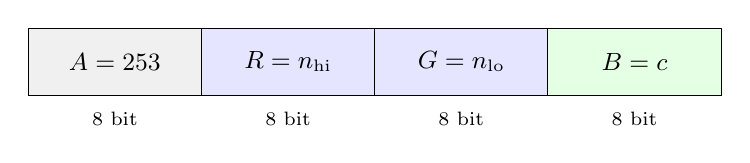
\begin{tikzpicture}[font=\small]
\fill[black!6] (0,0) rectangle (2.2,.85);
\fill[blue!10] (2.2,0) rectangle (6.6,.85);
\fill[green!10] (6.6,0) rectangle (8.8,.85);
\draw (0,0) rectangle (8.8,.85);
\foreach \x in {2.2,4.4,6.6} {\draw (\x,0) -- (\x,.85);}
\node at (1.1,.425) {$A=253$};
\node at (3.3,.425) {$R=n_{\mathrm{hi}}$};
\node at (5.5,.425) {$G=n_{\mathrm{lo}}$};
\node at (7.7,.425) {$B=c$};
\node[font=\scriptsize] at (1.1,-.3) {8 bit};
\node[font=\scriptsize] at (3.3,-.3) {8 bit};
\node[font=\scriptsize] at (5.5,-.3) {8 bit};
\node[font=\scriptsize] at (7.7,-.3) {8 bit};
\end{tikzpicture}
\end{document}
